\subsubsection{Numberlink (\ac{AKA} Flow Free) puzzle (Z3Py)}

You probably saw Flow Free puzzle:

\begin{figure}[H]
\centering
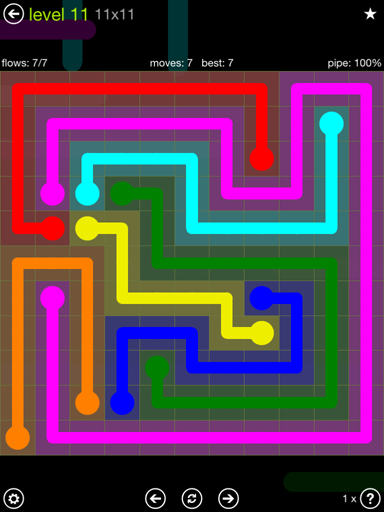
\includegraphics[scale=0.3]{puzzles/numberlink/Z3/flow-extreme-11-11.png}
\caption{}
\end{figure}

I'll stick to Numberlink version of the puzzle. This is the example puzzle from Wikipedia:

\begin{figure}[H]
\centering
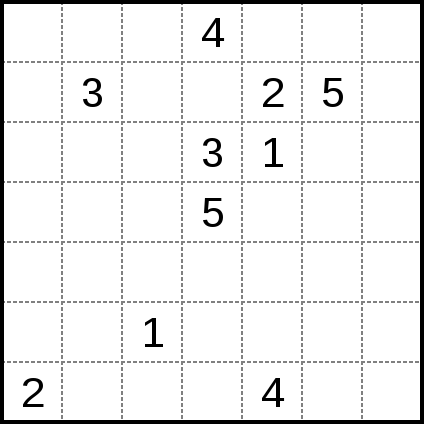
\includegraphics[scale=0.3]{puzzles/numberlink/Z3/424px-Numberlink_puzzle.svg.png}
\caption{}
\end{figure}

This is solved:

\begin{figure}[H]
\centering
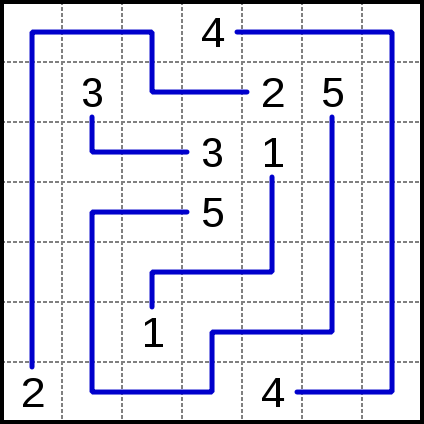
\includegraphics[scale=0.3]{puzzles/numberlink/Z3/424px-Numberlink_puzzle_solution.svg.png}
\caption{}
\end{figure}

See also:
\url{https://en.wikipedia.org/wiki/Numberlink},
\url{https://en.wikipedia.org/wiki/Flow_Free}.

The code:

\lstinputlisting[style=custompy]{puzzles/numberlink/Z3/numberlink.py}

The solution:

\lstinputlisting{puzzles/numberlink/Z3/solution.txt}

\begin{figure}[H]
\centering
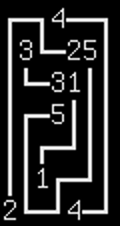
\includegraphics[scale=1]{puzzles/numberlink/Z3/solution.png}
\caption{The solution}
\end{figure}

